The SPS is equipped with a high bandwidth pick-up of approximately 2\,GHz allowing to resolve the intra-bunch motion. This instrument is called Head-Tail (HT) monitor and was originally designed for measuring chromaticity and transverse instabilities. However, in the SPS $\CC$ tests, the Head-Tail monitor was the main diagnostic device deployed for the demonstration of the crabbing and the measurement of the $\CC$ voltage (explained in details in Section~\ref{sec:CC_voltage_meas}). Therefore its use as a crabbing diagnostic should be explained here. The methods and procedures described in this section were developed at CERN and they are described here for the completeness of the thesis.

In the first part of this section some general information on the instrument along with example signals will be presented. Subsequently, the post processing of the Head-Tail signal in the presence of the $\CC$ will be discussed. Last, the calibration of the $\CC$ voltage from the Head-Tail data is described and the visualisation of the crabbing is displayed. The experimental data presented in this section were acquired, on May 30, 2018 (time-stamp: 13:51:05), at the SPS injection energy of 26\,GeV with only one $\CC$, $\CC$1, at phase $\phi_\mathrm{CC}=0$ (this means that the particle at the center of the bunch doesn't recieve any transverse deflection) for simplicity. That energy of 26\,GeV was chosen to provide a better understanding of the methods used as the orbit shift from the $\CC$ kick is stronger and thus more visible than at higher energies.

\section{General information}\label{subsec:HT_general_info}
As already mentioned, the Head-Tail monitor~\cite{sps_headtail_monitor} is a high bandwidth version of a standard beam position monitor, which means that it can measure the transverse displacement within the bunch. For reference it has a resolution of 100\,ps while the length of the bunches is $4\sigma_t \sim $2\,ns~\cite{Carver:2696108}.  This makes it ideal for the measurement of the intra-bunch offset caused from the $\CC$ kick. Its reading consists of the sum ($\Sigma$) and the  difference ($\Delta$) of the electrode signals of a straight stripline coupler (Fig.~\ref{fig:SPS_HT_diagram})~\cite{Jones:987561, Levens:2313358} over a defined acquisition period. The sum signal is the longitudinal line density while the difference signal corresponds to the intra-bunch offset. The system operates on timescales such that the signals are given as a function of the position within the bunch.

\begin{figure}[h]% Edit figure in: Goodle Docs/Doctoral/2022/Thesis/Ch4
   \centering         
   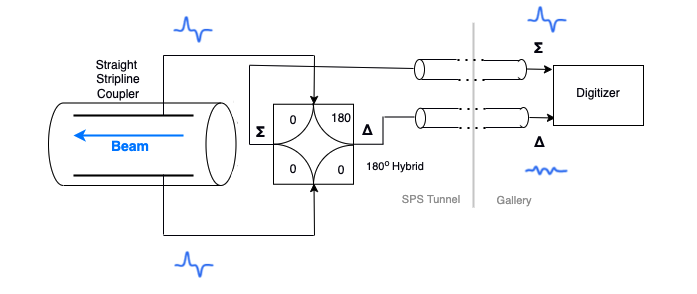
\includegraphics[width=1.0\textwidth]{images/Ch4/HT_monitor_sketch.png}
       \caption{Diagram of the SPS Head-Tail monitor~\cite{Levens:2313358}. The beam is passing through a straight stripline coupler which is followed by a 180$^\circ$hybrid. This configuration provides the sum ($\Sigma$) and the difference ($\Delta$) signal of the two electrodes.} %, which correspond to the longitudinal line density and intra-bunch offset, respectively.} 
       \label{fig:SPS_HT_diagram}
\end{figure}
% what is a 180 hybrid. A 180° Hybrid Coupler is a four port device that is used either to equally split an input signal with a 180° phase shift between the ports or to combine two signals that are 180° apart in phase. (from google)

The raw signals from the Head-Tail monitor require a specific post-processing procedure~\cite{Levens:2313358}, in order to provide useful information. Figure~\ref{fig:HT_example_signals} shows some example signals obtained from the Head-Tail monitor after the basic post-processing is applied. Moreover, Fig.~\ref{fig:HT_example_signals_2D} shows a 2D representation of the Head-Tail monitor reading. It is worth noting here that in the specific example a clear modulating pattern in time of the vertical intra-bunch offset (vertical $\Delta$) signal is observed. This is a result of the phase slip between the $\CC$ and the main RF system because they are not yet synchronised. 
% COMMENT: The Ref.~\cite{Levens:2313358} refers to the LHC HT monitor but the same applies for SPS as it is the same device.

\begin{figure}[!h]
   \centering         
   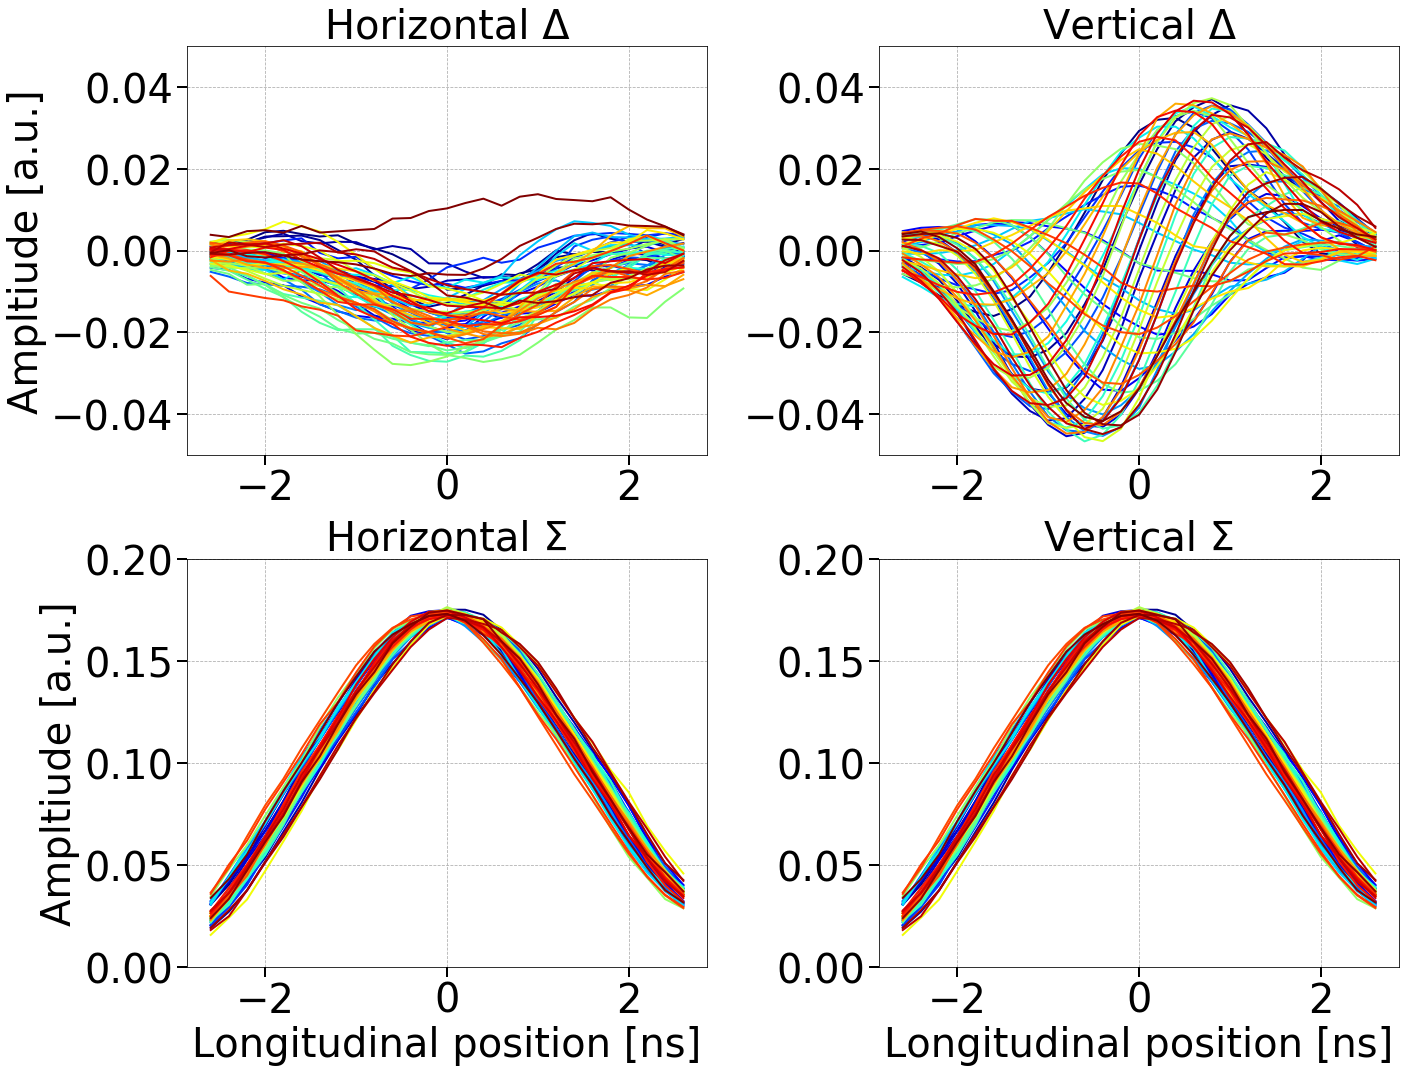
\includegraphics[width=0.8\textwidth]{images/Ch4/HT_1D__20180530_135105exampleAcq_4thesis_turnsStart0_Stop6000_step100_new.png}
       \caption{Example difference and sum signals (top and bottom plots, respectively) from the HT monitor, in time scale, with respect to the longitudinal position within the bunch over several SPS revolutions, after the basic post processing~\cite{Levens:2313358} but before the baseline correction. The different colors indicate the signals from different turns (every 100 turns). } % mention every how many turns you plot, shows an indication of how fast is the instrument.
       \label{fig:HT_example_signals}
\end{figure}
% /eos/user/n/natriant/2018/CC_MD_2018_summary/2018_HT_monitor/MD2_phase_scan_CC1/main_example_135105/plot_1example_HT_acquisition_for_thesis_30May2018-135105_for_thesis_sin_fit_forCh4_fixed_fcc_standard_post_processing_Ch4_3_1.ipynb


\begin{figure}[!h]
   \centering         
   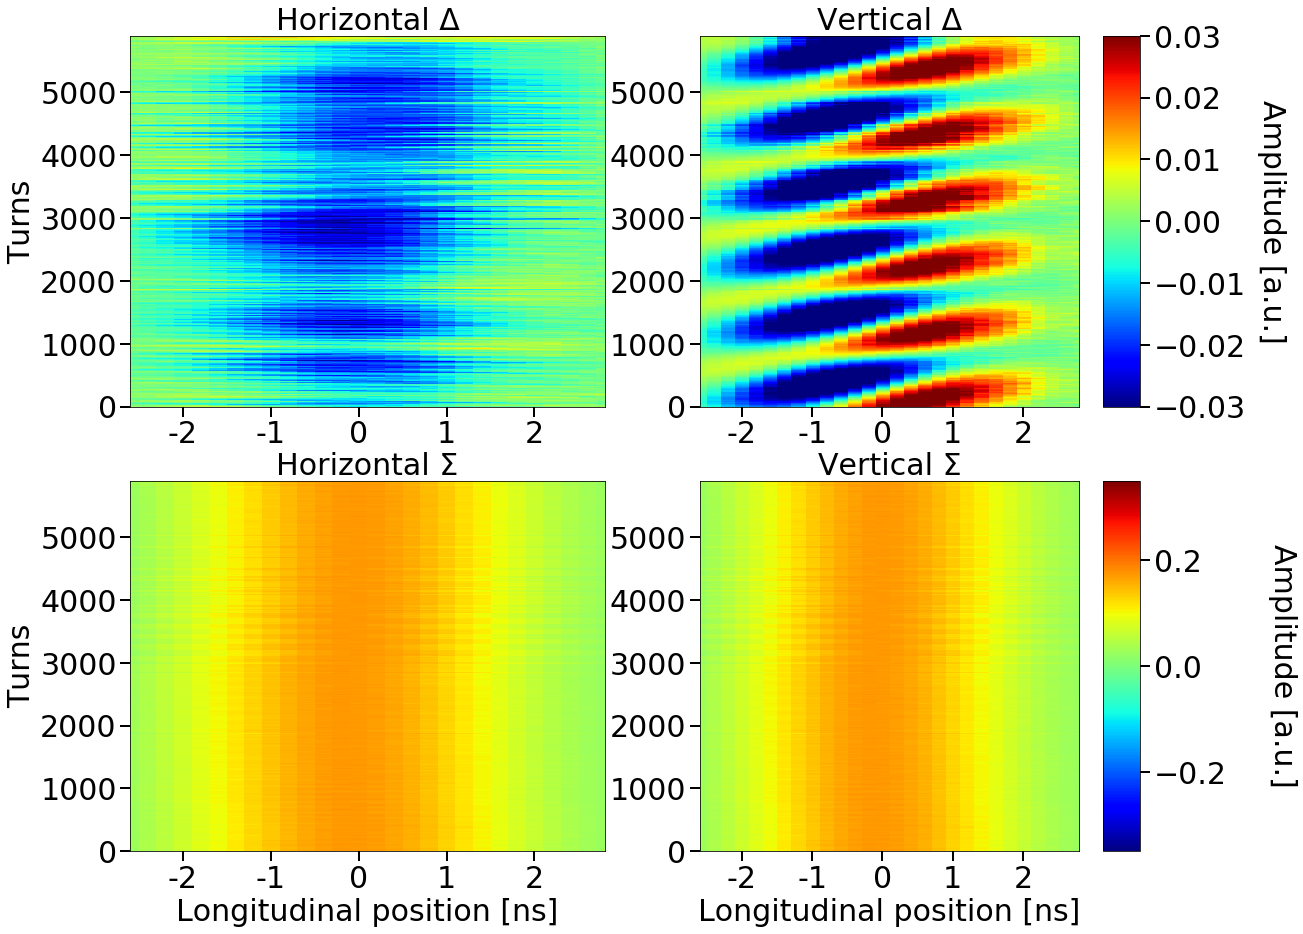
\includegraphics[width=0.9\textwidth]{images/Ch4/HT_2D__20180530_135105_colorbar_new_version.png}
       \caption{2D representation of example difference and sum signals with respect to the longitudinal position within the bunch obtained from the Head-Tail monitor over several SPS revolutions.}
       \label{fig:HT_example_signals_2D}
\end{figure}
% /eos/user/n/natriant/2018/CC_MD_2018_summary/2018_HT_monitor/MD2_phase_scan_CC1/main_example_135105/plot_1example_HT_acquisition_for_thesis_30May2018-135105_for_thesis_sin_fit_forCh4_fixed_fcc_standard_post_processing_Ch4_3_1.ipynb


\section{Post processing in the presence of Crab Cavities}\label{subsec:HT_post_process_CC}
To obtain useful information from the Head-Tail monitor signal in the presence of the $\CC$s there are a few steps that differ from the standard post processing procedure and they are desribed below.

\subsection{Head-Tail monitor baseline correction}\label{subsec:HT_baseline_correction}
The Head-Tai monitor measurement has a baseline on the difference signal which needs to be removed. The baseline is a result of orbit offsets and non-linearities of the instrument and is constant from turn to turn~\cite{Levens:2313358}. Therefore, during the normal post processing procedure (without $\CC$s), the baseline is computed as the mean of the difference signals over all turns and then the correction is achieved by subtracting this static offset from the signal of each turn. However, in the SPS tests, where the $\CC$s are well synchronised with the main RF system (Section~\ref{sec:cc_setup}), the crabbing signal is also a static intra-bunch position offset and thus would also be removed with the usual method. Because of technical limitations it was not feasible to switch off the $\CC$ for those kind of measurements. Thus, the following technique was used. 
% CC effect average out over time

For the $\CC$ experiments a reference measurement had first to be made with the $\CC$ not being synchronous with the main RF system. The baseline was computed as the mean of the difference signals over this reference period and subsequently it was subtracted from the average of the difference signals acquired after the synchronisation (Fig~\ref{fig:HT_baseline_correction}). The datasets before and after synchronisation are easily distinguishable in the 2D HT monitor reading as displayed in Fig.~\ref{fig:HT_baseline_correction_measurements_2D}.


% /eos/user/n/natriant/2018/CC_MD_2018_summary/2018_HT_monitor/MD2_phase_scan_CC1/main_example_135105/plot_1example_HT_acquisition_for_thesis_30May2018-135105_for_thesis_sin_fit_forCh4_fixed_fcc-CC_post_processing_Ch4_3_2_and_after.ipynb
\begin{figure}[!h]
   \centering         
   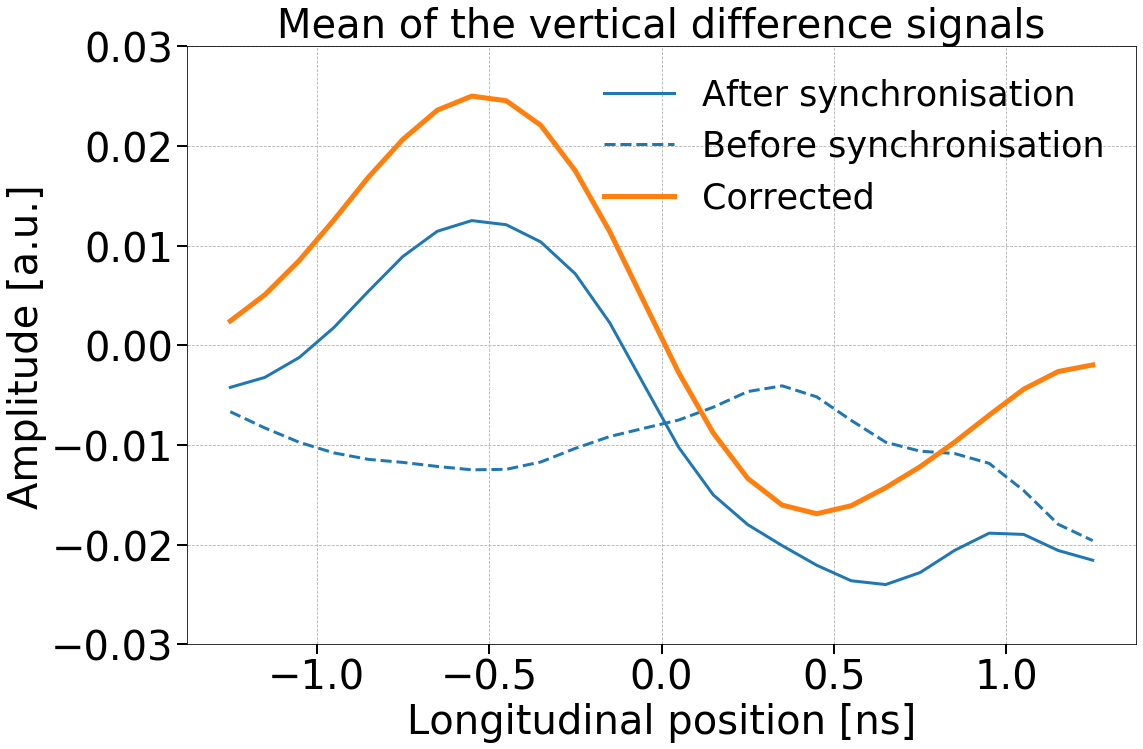
\includegraphics[width=0.65\textwidth]{images/Ch4/HT_measures_vs_reference_vs_corrected__20180530_135105_baseline_correction_new_version_CC_post_processing.png}
       \caption{HT monitor baseline correction for the SPS CC tests. The baseline signal (blue dashed line) refers to the mean of the difference signals acquired before the CC - main RF synchronisation. The measured signal (blue solid line) corresponds to the mean of the difference signal acquired after the synchronisation. Last, the corrected signal (orange solid line) is obtained after subtracting the baseline from the measured signal.}
       \label{fig:HT_baseline_correction}
\end{figure}

% /eos/user/n/natriant/2018/CC_MD_2018_summary/2018_HT_monitor/MD2_phase_scan_CC1/main_example_135105/plot_1example_HT_acquisition_for_thesis_30May2018-135105_for_thesis_sin_fit_forCh4_fixed_fcc_standard_post_processing_Ch4_3_1.ipynb
\begin{figure}[!h]
    \centering         
    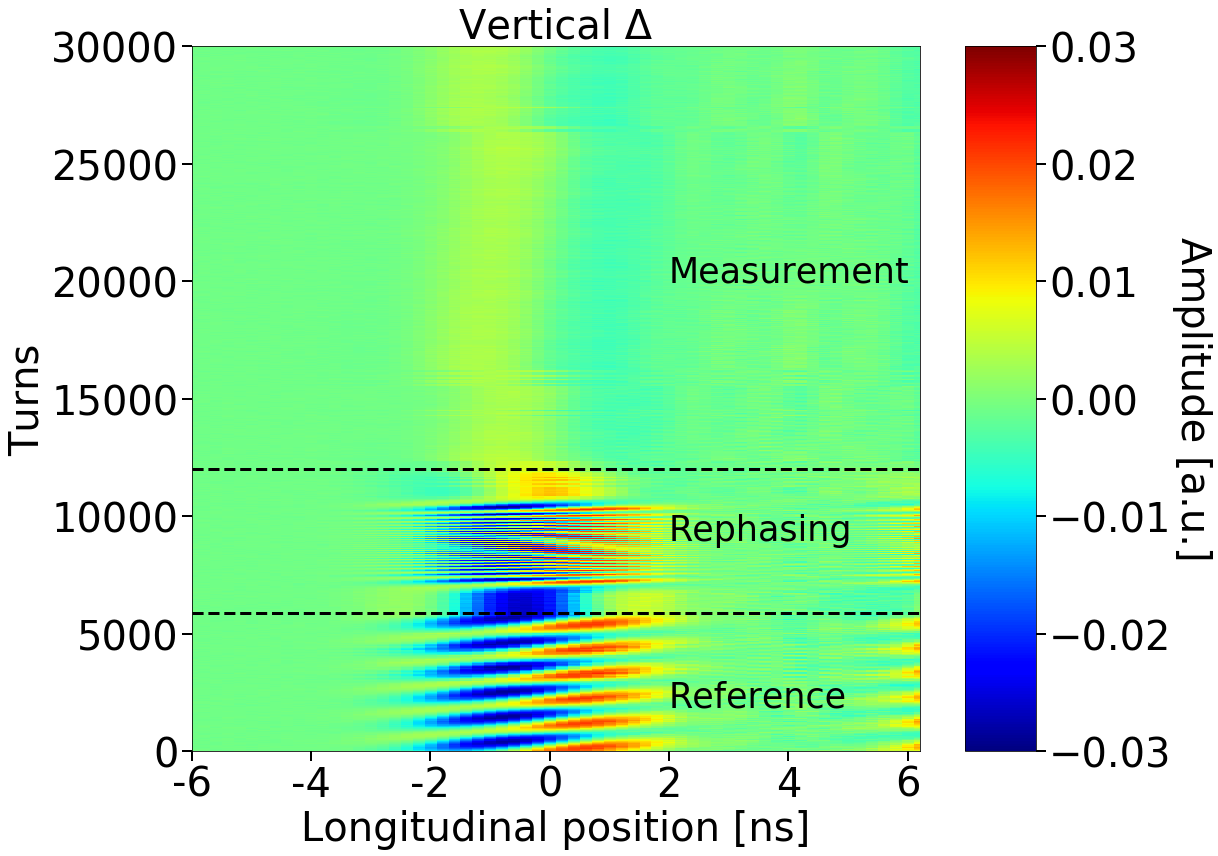
\includegraphics[width=0.7\textwidth]{images/Ch4/HT_2D__20180530_135105_before_after_sunchronisation_new_version.png}
        \caption{HT acquistions before and after the synchronisation of the SPS main RF with the CC.}
        \label{fig:HT_baseline_correction_measurements_2D}
 \end{figure}


%At this point, it should be mentioned that the baseline (blue dashed line in Fig.~\ref{fig:HT_baseline_correction}) appears to vary with position within the bunch. The origin for this is not yet understood and will have to be addressed in the future to fully understand .... However, here is our working assumption ...

\normalsize{\textbf{Head-Tail monitor scaling}}\\
The last step to make the HT acquisitions meaningful is to convert the measured intra bunch offset (the mean of the difference signals following phase synchronisation and baseline correction) from arbitrary units to millimeters. The scaling is achieved by dividing by the mean of the sum signals (which is a function of the position along the bunch and is calculated for each point individually over many turns) after the synchronisation and with a normalisation factor which is provided by the calibration of the HT monitor~\cite{PhysRevAccelBeams.22.112803}. The normalisation factor for the SPS was measured at 0.1052 in 2018~\cite{HT_calibration_2018}. Figure~\ref{fig:HT_baseline_correction_crabbing_mm} shows the intra-bunch offset from the $\CC$ kick in millimeters and after the baseline correction. 

% /eos/user/n/natriant/2018/CC_MD_2018_summary/2018_HT_monitor/MD2_phase_scan_CC1/main_example_135105/plot_1example_HT_acquisition_for_thesis_30May2018-135105_for_thesis_sin_fit_forCh4_fixed_fcc-CC_post_processing_Ch4_3_2_and_after.ipynb
\begin{figure}[!h]
   \centering         
   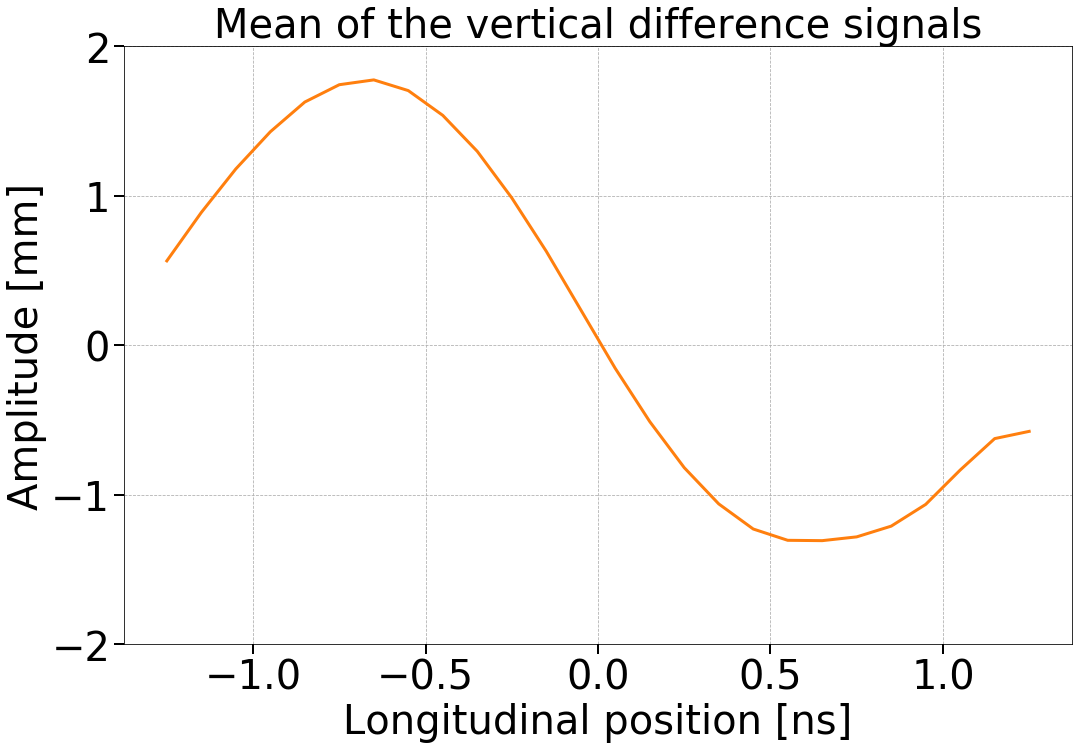
\includegraphics[width=0.65\textwidth]{images/Ch4/HT_corrected__20180530_135105_baseline_correction_new_version_CC_post_processing.png}
       \caption{Intra-bunch offset from the CC kick expressed in millimeters after the removal of the baseline.}
       \label{fig:HT_baseline_correction_crabbing_mm}
\end{figure}


 \subsection{Crab Cavity voltage reconstruction}\label{sec:Vcc_calibration}
 This section discusses the reconstruction of the $\CC$ voltage from the HT monitor signal. First, Eq.~\eqref{eq:CC_orbit_shift_Chao} was used to calculate the $\CC$ kick, $\theta$, required to reconstruct the measured intra-bunch offset. Equation~\eqref{eq:CC_orbit_shift_Chao}, which is obtained from Eq.\,(1) from chapter 4.7.1 in Ref.~\cite{Chao:1490001}, gives the vertical orbit shift (in meters) from the $\CC$ kick, $\theta$, at the HT monitor location as follows:

\begin{equation}\label{eq:CC_orbit_shift_Chao}
   \Delta y_{,HT} = \frac{\sqrt{\beta_{y, HT}}}{2 \sin(\pi \Qy)} \theta \sqrt{\beta_{y, CC}} \cos(\pi \Qy - \mid \psi_{y, HT} - \psi_{y, CC} \mid),
\end{equation}

where $\beta_y$ is the beta function, $\Qy$ is the tune, and $\mid \psi_{y, HT} - \psi_{y, CC} \mid$ is the vertical phase advance (in tune units) between the $\CC$ and the HT monitor. The same applies for the horizontal plane. The subscripts HT and CC indicate quanities at the location of the HT monitor and CC respectively.

The $\CC$ voltage is then reconstructed from the $\CC$ kick which is written as $\theta = - \frac{q V_{CC}(t)}{\symE}$, where $q$ is the charge of the particle, $\symE$ the beam energy and $V_{CC}(t) = \VCC \sin(2 \pi \fCC t + \phiCC) $ is the voltage that a particle experiences while passing through the $\CC$. In the context where the HT monitor measures the signal as a function of time, $t$, the voltage in the above formula is expressed accordingly as $V_{CC}(t)$, where $t=0$ the center of the bunch.

% 1. locally PhD_projects/CC_MD_2021_summary/HT_monitor/2018_HT_monitor/MD2_phase_scan
% /eos/user/n/natriant/2018/CC_MD_2018_summary/2018_HT_monitor/MD2_phase_scan_CC1/main_example_135105/plot_1example_HT_acquisition_for_thesis_30May2018-135105_for_thesis_sin_fit_forCh4_fixed_fcc-CC_post_processing_Ch4_3_2_and_after.ipynb
\begin{figure}[!h]
\centering         
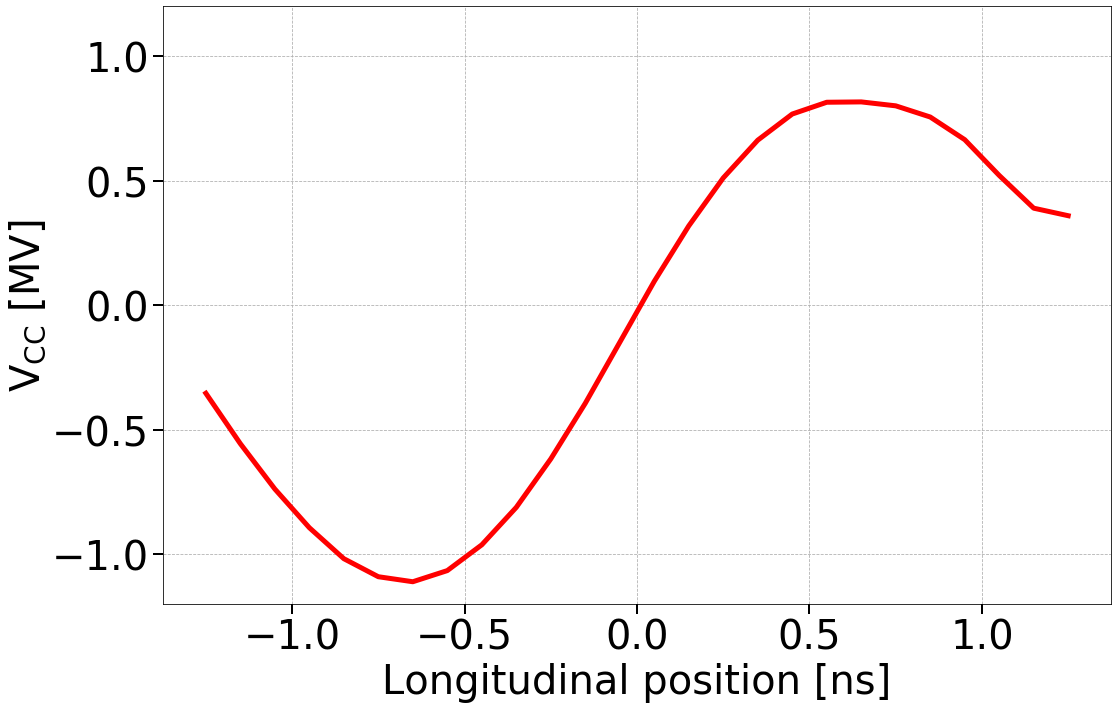
\includegraphics[width=0.65\textwidth]{images/Ch4/HT_VCC_callibration_20180530_135105_CC_post_processing.png}
    \caption{CC voltage reconstruction from the HT monitor.}
    \label{fig:VCC_from_HT_monitor_measurement}
\end{figure}

It should be noted here, that the measured intra-bunch offset, $\Delta y_{, HT}$, is inserted in Eq.~\eqref{eq:CC_orbit_shift_Chao} after removing the baseline and converting it to millimeters as discussed in Section~\ref{subsec:HT_post_process_CC}. Figure~\ref{fig:VCC_from_HT_monitor_measurement} illustrates the cavity voltage computed from the HT signals shown already in this section. The corresponding beam and optic parameters are listed in Table~\ref{tab:SPS_HT_CC}.

% optics at CC1, CC2 and HT monitor location /eos/user/n/natriant/Project_thesis/SPS optics
\begin{table}[!hbt]
	\begin{minipage}{\textwidth}
   \begin{centering}
   \caption{Parameters for computing the CC voltage from the example HT monitor measurements discussed in this chapter.}
	\begin{tabu} to \textwidth {X[c,m] X[0.01c,m] X[0.01c,m] X[0.01c,m]}
		&&& \\[-6mm]
		\toprule \toprule
		\multicolumn{2}{l}{\textbf{Parameter}} &
		\multicolumn{2}{c}{\textbf{Value}} \\
		\bottomrule
      \multicolumn{2}{l}{Beta function at the HT monitor, $\beta_{y, HT}$}& \multicolumn{2}{c}{49.19\,m} \\
      \multicolumn{2}{l}{Phase advance to the HT monitor$^{\ast}$, $\psi_{y, HT}$} & \multicolumn{2}{c}{15.68 $\times$ 2$\mathrm{\pi}$} \\
      \multicolumn{2}{l}{Beta function at the $\CC$1, $\beta_{y, CC1}$}& \multicolumn{2}{c}{76.07\,m} \\
      \multicolumn{2}{l}{Phase advance to the $\CC$1$^{\ast}$, $\psi_{y, CC1}$} & \multicolumn{2}{c}{23.9 $\times$ 2$\mathrm{\pi}$} \\
      \multicolumn{2}{l}{Vertical betatron tune, $\Qy$} & \multicolumn{2}{c}{26.18} \\
      \multicolumn{2}{l}{Beam energy, $\symE$} & \multicolumn{2}{c}{26\,GeV} \\
      \bottomrule
	\end{tabu}
   \label{tab:SPS_HT_CC}
   \end{centering} \footnotesize{$^\ast$ The phase advances are measured from the start of the lattice which is considered the element QF.10010 that is a focusing quadrupole.}
   \end{minipage}
\end{table}

\subsection{Demonstration of crabbing with proton beams}\label{subsec:crabbing_demonstration_density_plot}
Additionally, the measurements from the HT monitor were used for reconstructing the crabbing and representating schematically the beam projection in the transverse plane. The technique for reconstructing the crabbing was developed at CERN in 2018 and was extensively used throughout the experimental campaign with $\CC$s since (together with the calibrated voltage) it gives a straightforward estimate of the applied $\CC$ kick, as illustrated in Fig.~\ref{fig:crabbing_reconstruction_HT_monitor}. 

To obtain this schematic representation, which in practice is a density plot showing the effect of the $\CC$ kick on the beam, one needs to multiply the measured longitudinal profile (the mean of the sum signals acquired after phase synchronisation) with the measured intra-bunch offset, mean of the difference signals acquired after the synchronisation. An example of this is shown in Fig.~\ref{fig:HT_baseline_correction_crabbing_mm}. For the transverse plane a gaussian distribution is considered with $\sigma$ obtained from the wire scanner (addressed in more detail in the following section). The color code of Fig.~\ref{fig:crabbing_reconstruction_HT_monitor} is normalised to the maximum intensity within the bunch.

% /eos/user/n/natriant/2018/CC_MD_2018_summary/2018_HT_monitor/MD2_phase_scan_CC1/main_example_135105/plot_1example_HT_acquisition_for_thesis_30May2018-135105_for_thesis_sin_fit_forCh4_fixed_fcc-CC_post_processing_Ch4_3_2_and_after.ipynb
\begin{figure}[!h]
   \centering         
   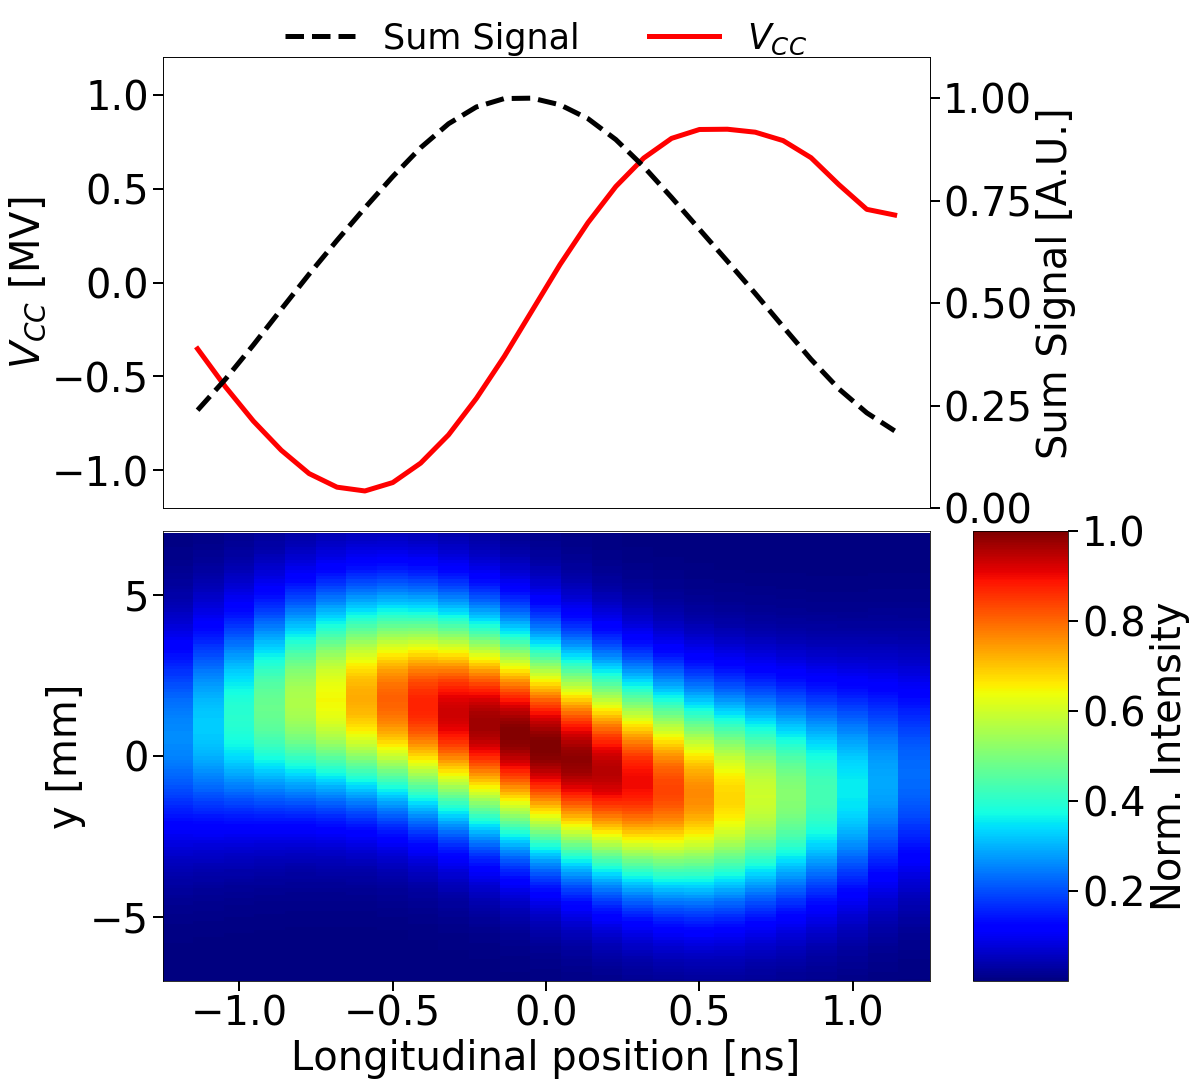
\includegraphics[width=0.7\textwidth]{images/Ch4/HT_crabVoltage__20180530_135105_crabbing_only_CC_post_processing.png}
       \caption{Demonstration of the crabbing from the HT monitor signal. CC voltage and sum signal (longitudinal line density) measured from the HT monitor (top) together with the density plot (bottom) which visualises the effect of the CC kick on the beam.}
       \label{fig:crabbing_reconstruction_HT_monitor}
\end{figure}
   
